% Copyright (c) 2022 by Lars Spreng
% This work is licensed under the Creative Commons Attribution 4.0 International License. 
% To view a copy of this license, visit http://creativecommons.org/licenses/by/4.0/ or send a letter to Creative Commons, PO Box 1866, Mountain View, CA 94042, USA.

%~~~~~~~~~~~~~~~~~~~~~~~~~~~~~~~~~~~~~~~~~~~~~~~~~~~~~~~~~~~~~~~~~~~~~~~~~~~~~~
% You can add your packages and commands to the loadslides.tex file. 
% The files in the folder "styles" can be modified to change the layout and design of your slides.
% I have included examples on how to use the template below. 
% Some of these examples are taken from the Metropolis template.
%~~~~~~~~~~~~~~~~~~~~~~~~~~~~~~~~~~~~~~~~~~~~~~~~~~~~~~~~~~~~~~~~~~~~~~~~~~~~~~


\documentclass[
11pt,notheorems,hyperref={pdfauthor=whatever}
]{beamer}


% Copyright (c) 2022 by Lars Spreng
% This work is licensed under the Creative Commons Attribution 4.0 International License. 
% To view a copy of this license, visit http://creativecommons.org/licenses/by/4.0/ or send a letter to Creative Commons, PO Box 1866, Mountain View, CA 94042, USA.

%~~~~~~~~~~~~~~~~~~~~~~~~~~~~~~~~~~~~~~~~~~~~~~~~~~~~~~~~~~~~~~~~~~~~~~~~~~~~~~
% Add your packages and commands to this file
%~~~~~~~~~~~~~~~~~~~~~~~~~~~~~~~~~~~~~~~~~~~~~~~~~~~~~~~~~~~~~~~~~~~~~~~~~~~~~~

%~~~~~~~~~~~~~~~~~~~~~~~~~~~~~~~~~~~~~~~~~~~~~~~~~~~~~~~~~~~~~~~~~~~~~~~~~~~~~~
% Fonts
% \RequirePackage{palatino} % for serif slides
% \usefonttheme{serif}
\RequirePackage[scaled]{helvet} % for sans-serif slides

\RequirePackage[utf8]{inputenc}
\RequirePackage[T1]{fontenc}


\usepackage{styles/elegantmacros}
\usefolder{styles}
\usetheme[style=lecture]{elegant}

\newcommand{\makepart}[1]{ % For convenience
\part{#1} \frame{\partpage}
}

%~~~~~~~~~~~~~~~~~~~~~~~~~~~~~~~~~~~~~~~~~~~~~~~~~~~~~~~~~~~~~~~~~~~~~~~~~~~~~~

%~~~~~~~~~~~~~~~~~~~~~~~~~~~~~~~~~~~~~~~~~~~~~~~~~~~~~~~~~~~~~~~~~~~~~~~~~~~~~~
% Figures
\RequirePackage{booktabs}
\RequirePackage{colortbl}
\RequirePackage{ragged2e}
\RequirePackage{schemabloc}
%\RequirePackage{natbib}
\RequirePackage{caption}
\RequirePackage{subcaption}
\RequirePackage{tabularx}
\RequirePackage{array}
\RequirePackage{multirow}
\RequirePackage[%
  natbib=true, backend=biber,%
  style=apa, isbn=false,url=false,uniquename=false%, useprefix=true%
  ]{biblatex}
\addbibresource{references.bib}
\newcolumntype{Y}{>{\centering\arraybackslash}X}

%~~~~~~~~~~~~~~~~~~~~~~~~~~~~~~~~~~~~~~~~~~~~~~~~~~~~~~~~~~~~~~~~~~~~~~~~~~~~~~

%~~~~~~~~~~~~~~~~~~~~~~~~~~~~~~~~~~~~~~~~~~~~~~~~~~~~~~~~~~~~~~~~~~~~~~~~~~~~~~
% Figures
\RequirePackage{wrapfig}
\RequirePackage{pgfplots}
\RequirePackage{graphicx}
\RequirePackage{adjustbox}
\RequirePackage{environ}
\pgfplotsset{compat=1.18}

\makeatletter
\newsavebox{\measure@tikzpicture}
\NewEnviron{scaletikzpicturetowidth}[1]{%
  \def\tikz@width{#1}%
  \def\tikzscale{1}\begin{lrbox}{\measure@tikzpicture}%
  \BODY
  \end{lrbox}%
  \pgfmathparse{#1/\wd\measure@tikzpicture}%
  \edef\tikzscale{\pgfmathresult}%
  \BODY
}
\makeatother
%~~~~~~~~~~~~~~~~~~~~~~~~~~~~~~~~~~~~~~~~~~~~~~~~~~~~~~~~~~~~~~~~~~~~~~~~~~~~~~

%~~~~~~~~~~~~~~~~~~~~~~~~~~~~~~~~~~~~~~~~~~~~~~~~~~~~~~~~~~~~~~~~~~~~~~~~~~~~~~
% Maths 
\RequirePackage{textcomp}
\RequirePackage{amsmath} 
\RequirePackage{amsthm}
\RequirePackage{mathtools}
%\RequirePackage{bbm}
%\RequirePackage{algorithm}
%\RequirePackage[osf,sc]{mathpazo}
%\RequirePackage{pifont}
%\newcommand{\xmark}{\ding{55}}%
%\numberwithin{equation}{section}
\DeclareMathOperator*{\argmax}{arg\,max}
\DeclareMathOperator*{\argmin}{arg\,min}

\setbeamertemplate{theorems}[numbered] % to number

\theoremstyle{definition}
\newtheorem{fact}{Fact}[section]
\newtheorem{examp}{Example}[section]

\theoremstyle{plain}
\newtheorem{definition}{Definition}[section]
\newtheorem{proposition}{Proposition}
\newtheorem{theorem}{Theorem}
\newtheorem{assumption}{Assumption}

\providecommand{\H}{\mathscr{H}}      
\providecommand{\E}{\mathbb{E}}
\makeatletter
\def\munderbar#1{\underline{\sbox\tw@{$#1$}\dp\tw@\z@\box\tw@}}
\makeatother

%~~~~~~~~~~~~~~~~~~~~~~~~~~~~~~~~~~~~~~~~~~~~~~~~~~~~~~~~~~~~~~~~~~~~~~~~~~~~~~
 % Loads packages and some defined commands

\title[
% Text entered here will appear in the bottom middle
]{Toom-Cook Multiplication and Toom-Cook TMVP}

\subtitle{Mathematical Description with SageMath Demonstration}

\author[
% Text entered here will appear in the bottom left corner
Cesare
]{
    Cesare Huang Cheng Wei 
}

\institute{
    Author Affiliation, \\
    University of Author}
\date{\today}

\begin{document}

% Generate title page
{
\setbeamertemplate{footline}{} 
\begin{frame}
  \titlepage
\end{frame}
}
\addtocounter{framenumber}{-1}

% You can declare different parts as a parentof sections
\begin{frame}{Part I: Toom-Cook Multiplication}
    \tableofcontents[part=1]
\end{frame}
\begin{frame}{Part II: Toom-Cook TMVP}
    \tableofcontents[part=2]
\end{frame}

\makepart{Toom-Cook Multiplication}

\section{Idea of Toom-Cook-3 Multiplication}
\subsection{Motivation}
\begin{frame}
    We want to compute the product $R(x)$ of degree $2$ (length $3$) polynomials $B(x)$ and $C(x)$. 

    Denote the polynomials by column vectors: If $B(x) = B_{0} + B_{1}x+B_{2}x^{2}$, $C(x) = C_{0} + C_{1}x + C_{2} x^{2}$ and $R(x) = R_{0} + R_{1}x+R_{2}x^{2} + R_{3} x^{3} + R_{4} x^{4}$ then 
    \[
        B(x) = \begin{bmatrix} B_{0} \\ B_{1} \\ B_{2} \end{bmatrix}
        ,
        C(x) = \begin{bmatrix} C_{0} \\ C_{1} \\ C_{2} \end{bmatrix}
        \text{ and }
        R(x) = \begin{bmatrix} R_{0} \\ R_{1} \\ R_{2} \\ R_{3} \\ R_{4} \end{bmatrix}
    \]
\end{frame}

\begin{frame}
    Since the result $R$ has five coefficients, we can determine the polynomial $R$ by five function values $R(s_{i})$ for $i=0,...,4$.
    This proccess is also known as "interpolation".

    These function values
    \[R(s_{i}) = B(s_{i})C(s_{i})\]
    can be computed by function values of polynomial $B$ and $C$.

    And the function values $B(s_{i})$ and $C(s_{i})$ can be determined by simply evaluate polynomials $B$ and $C$ at $s_{i}$'s.
\end{frame}

\begin{frame}
    So far, we obtained a method to multiply polynomials:
    \begin{enumerate}
        \item Evaluate $B$ and $C$ at $5$ points,  $\{ s_{i} \}$.
        \item Compute $R(s_{i}) = B(s_{i}) \cdot C(s_{i})$ for $i=0,...,4$.
        \item Interpolate $R$ from the data $R(s_{i})$'s.
    \end{enumerate}

    These are the idea of Toom-Cook-3 multiplication.
    Let's dive into the detailed steps.
\end{frame}


\subsection{Detailed Steps}

\begin{frame}
    Our first step is "Evaluate $B$ and $C$ at $5$ points, $\{ s_{i} \}$".
    And we choose $\{s_{i}\} = \{0,1,-1,2,\infty\}$.

    Here, $P(\infty)$ is defined as the leading coefficient of polynomial $P$.

    This can be done by using the evaluation transform (matrix)\footnote[]{Evaluation is itself a linear operation hence we can naturally write it as a matrix multiplication.}:
    \[
    \left[\begin{array}{l}
    B(0) \\
    B(1) \\
    B(-1) \\
    B(2) \\
    B(\infty)
    \end{array}\right]=\left[\begin{array}{ccc}
    1 & 0 & 0 \\
    1 & 1 & 1 \\
    1 & -1 & 1 \\
    1 & 2 & 4 \\
    0 & 0 & 1
    \end{array}\right]\left[\begin{array}{l}
    B_0 \\
    B_1 \\
    B_2
    \end{array}\right]
    \]
\end{frame}

\begin{frame}
    We will from now on denote the matrices of evaluations by $\mathbf{TC}$'s.
    \[
    \mathbf{TC}_{5\times 3}=\left[\begin{array}{ccc}
    1 & 0 & 0 \\
    1 & 1 & 1 \\
    1 & -1 & 1 \\
    1 & 2 & 4 \\
    0 & 0 & 1
    \end{array}\right], \quad \mathbf{TC}_{5 \times 5}=\left[\begin{array}{ccccc}
    1 & 0 & 0 & 0 & 0 \\
    1 & 1 & 1 & 1 & 1 \\
    1 & -1 & 1 & -1 & 1 \\
    1 & 2 & 4 & 8 & 16 \\
    0 & 0 & 0 & 0 & 1
    \end{array}\right]
    \]
    So that 
    \[
    \left[\begin{array}{l}
    B(0) \\
    B(1) \\
    B(-1) \\
    B(2) \\
    B(\infty)
    \end{array}\right]=\mathbf{TC}_{5\times 3}\left[\begin{array}{l}
    B_0 \\
    B_1 \\
    B_2
    \end{array}\right]\text{ and importantly }
    \left[\begin{array}{l}
        R(0) \\
        R(1) \\
        R(-1) \\
        R(2) \\
        R(\infty)
        \end{array}\right] = \mathbf{TC}_{5\times 5}
    \left[\begin{array}{l}
        R_0 \\
        R_1 \\
        R_2 \\
        R_3 \\
        R_4
        \end{array}\right]
    \]
\end{frame}

\begin{frame}
    Nextly, we do "Compute $R(s_{i}) = B(s_{i}) \cdot C(s_{i})$ for $i=0,...,4$"
    \[
    \left[\begin{array}{l}
    R(0) \\
    R(1) \\
    R(-1) \\
    R(2) \\
    R(\infty)
    \end{array}\right]=\left[\begin{array}{l}
    B(0)C(0)   \\
    B(1)C(1)   \\
    B(-1)C(-1) \\
    B(2)C(2)   \\
    B(\infty)C(\infty)
    \end{array}\right]=\left[\begin{array}{l}
    B(0) \\
    B(1) \\
    B(-1) \\
    B(2) \\
    B(\infty)
    \end{array}\right] \odot\left[\begin{array}{l}
    C(0) \\
    C(1) \\
    C(-1) \\
    C(2) \\
    C(\infty)
    \end{array}\right]
    \]
    where $\odot$ denote the component-wise multiplication.

    By using the matrices defined in the previous page, we can write the above equation as
    \[
    \mathbf{TC}_{5 \times 5} R=\left(\mathbf{TC}_{5 \times 3} B\right) \odot\left(\mathbf{TC}_{5 \times 3} C\right)
    \]
\end{frame}

\begin{frame}
    The last step is "Interpolate $R$ from the data $R(s_{i})$'s"

    By the equation we just wrote
    \[
    \mathbf{TC}_{5 \times 5} R=\left(\mathbf{TC}_{5 \times 3} B\right) \odot\left(\mathbf{TC}_{5 \times 3} C\right)
    \]
    this step is simply multiply both sides by $\mathbf{TC}_{5 \times 5}^{-1}$:
    \[
    \begin{aligned}
    \mathbf{TC}_{5 \times 5}^{-1}\left(\mathbf{TC}_{5 \times 5} R\right) & =\mathbf{TC}_{5 \times 5}^{-1}\left(\left(\mathbf{TC}_{5 \times 3} B\right) \odot\left(\mathbf{TC}_{5 \times 3} C\right)\right) \\
    R & =\mathbf{TC}_{5 \times 5}^{-1}\left(\left(\mathbf{TC}_{5 \times 3} B\right) \odot\left(\mathbf{TC}_{5 \times 3} C\right)\right) .
    \end{aligned}
    \]
    Completes the computation.

\end{frame}

\begin{frame}
    \[
        R =\textcolor{blue}{\mathbf{TC}_{5 \times 5}^{-1}}
        \left(
            \left(
                \textcolor{red}{\mathbf{TC}_{5 \times 3}} B
            \right) \textcolor{cyan}{\odot}\left(
                \textcolor{red}{\mathbf{TC}_{5 \times 3}} C
            \right)
        \right) .
    \]
    \begin{enumerate}
        \item \textcolor{red}{Evaluate $B$ and $C$ at $5$ points,  $\{ s_{i} \}$.}
        \item \textcolor{cyan}{Compute $R(s_{i}) = B(s_{i}) \cdot C(s_{i})$ for $i=0,...,4$.}
        \item \textcolor{blue}{Interpolate $R$ from the data $R(s_{i})$'s.}
    \end{enumerate}
\end{frame}

\subsection{Demo for Toom-Cook-3}

\begin{frame}
    We use SageMath
\end{frame}

\section{Idea of Toom-Cook-$k$ Multiplication}
\begin{frame}
We can generalize the notion of Toom-Cook-3 into Toom-Cook-$k$.

We want to compute the product $R(x)$ of degree $k-1$ (length $k$) polynomials $B(x)$ and $C(x)$.
Since the result $R(x)$ is of degree at most $2k-2$, we can interpolate $R(x)$ by $2k-1$ function values.
\end{frame}
\subsection{Detailed Steps}
\begin{frame}
    The steps are similar to Toom-Cook-3 multiplication:
    \begin{enumerate}
        \item Evaluate $B$ and $C$ at $2k-1$ points, $\{ s_{i} \}$.
        \item Compute $R(s_{i}) = B(s_{i}) \cdot C(s_{i})$ for $i=0,...,2k-2$.
        \item Interpolate $R$ from the data $R(s_{i})$'s.
    \end{enumerate}
\end{frame}

\begin{frame}
    \[
        R =\textcolor{blue}{\mathbf{TC}_{(2k-1) \times (2k-1)}^{-1}}
        \left(
            \left(
                \textcolor{red}{\mathbf{TC}_{(2k-1) \times k}} B
            \right) \textcolor{cyan}{\odot}\left(
                \textcolor{red}{\mathbf{TC}_{(2k-1) \times k}} C
            \right)
        \right) .
    \]
    \begin{enumerate}
        \item \textcolor{red}{Evaluate $B$ and $C$ at $2k-1$ points,  $\{ s_{i} \}$.}
        \item \textcolor{cyan}{Compute $R(s_{i}) = B(s_{i}) \cdot C(s_{i})$ for $i=0,...,2k-2$.}
        \item \textcolor{blue}{Interpolate $R$ from the data $R(s_{i})$'s.}
    \end{enumerate}
\end{frame}

\subsection{Detail for Toom-Cook-5}
\begin{frame}
So far, we have not made some description on choosing $\{s_{i}\}$'s. 
In principal, $\{s_{i}\}$'s are chosen such that the computation of $\mathbf{TC}$'s are cheap.

Hence we select $\{0,1,-1,2,\infty\}$ in Toom-Cook-3 and the resulting $\mathbf{TC}$'s involve only addition/subtraction and multiplication by powers of 2.
And its inverse:
\[
\mathbf{TC}_{5\times 5}^{-1}=
    \left(\begin{array}{rrrrr}
        1 & 0 & 0 & 0 & 0 \\ \\
        -\frac{1}{2} & 1 & -\frac{1}{3} & -\frac{1}{6} & 2 \\ \\
        -1 & \frac{1}{2} & \frac{1}{2} & 0 & -1 \\ \\
        \frac{1}{2} & -\frac{1}{2} & -\frac{1}{6} & \frac{1}{6} & -2 \\ \\
        0 & 0 & 0 & 0 & 1
    \end{array}\right)
\]
are also simple (excepts the division by 3).

But the situation is not trivial when we need more interpolation points.
Hence we spend a subsection on Toom-Cook-5 multiplication.
\end{frame}    

\begin{frame}
    In Toom-Cook-5 multiplication, we need $9$ interpolation points.
    A naive choice is $\{s_{i}\} = \{0, 1, -1, 2, -2, 3, -3, 4, \infty \}$.
    But then the resulting $\mathbf{TC}$ matrices will have very large entries.

    Now, the choise in the paper is $\{s_{i}\} = \left\{0,1,-1,2,-2,3,\frac{1}{2},-\frac{1}{2},\infty\right\}$.
    A naive understanding of this will say that in the first step, the interpolation data
    $$
\left[\begin{array}{c}
\vdots \\
B\left(\frac{1}{2}\right) \\
B\left(-\frac{1}{2}\right) \\
\vdots
\end{array}\right]=\left[\begin{array}{ccccc} 
\vdots &\vdots &\vdots &\vdots &\vdots \\
1 & \frac{1}{2} & \frac{1}{4} & \frac{1}{8} & \frac{1}{16} \\
1 & -\frac{1}{2} & \frac{1}{4} & -\frac{1}{8} & \frac{1}{16}\\
\vdots & \vdots &\vdots &\vdots &\vdots 
\end{array}\right]\left[\begin{array}{c}
B_0 \\
B_1 \\
B_2 \\
B_3 \\
B_4
\end{array}\right]
$$
    are computed. 
    However, this produces division in the matrix. 
    

\end{frame}

\begin{frame}
    So we will instead evaluate $2^4 B(\frac{1}{2})$ and $(-2)^{4} B(-\frac{1}{2})$:
    $$
    \left[\begin{array}{c}
    \vdots \\
    2^4B\left(\frac{1}{2}\right) \\
    (-2)^4B\left(-\frac{1}{2}\right) \\
    \vdots
    \end{array}\right]=\left[\begin{array}{ccccc} 
    \vdots &\vdots &\vdots &\vdots &\vdots \\
    16 & 8 & 4 & 2 & 1 \\
    16 & -8 & 4 & -2 & 1 \\
    \vdots & \vdots &\vdots &\vdots &\vdots 
    \end{array}\right]\left[\begin{array}{c}
    B_0 \\
    B_1 \\
    B_2 \\
    B_3 \\
    B_4
    \end{array}\right]
    $$
\end{frame}

\begin{frame}
    The component-wise multiplication will yield
    \[
    \left[\begin{array}{c}
        \vdots \\
        2^8 R\left(\frac{1}{2}\right) \\
        (-2)^8 R\left(-\frac{1}{2}\right) \\
        \vdots
    \end{array}\right]=
    \left[\begin{array}{c}
        \vdots \\
        2^4B\left(\frac{1}{2}\right) \\
        (-2)^4B\left(-\frac{1}{2}\right) \\
        \vdots
    \end{array}\right]
    \odot
    \left[\begin{array}{c}
            \vdots \\
            2^4C\left(\frac{1}{2}\right) \\
            (-2)^4C\left(-\frac{1}{2}\right) \\
            \vdots
    \end{array}\right]
    \]
    and the final interpolation matrix will be
    $$
    \left[\begin{array}{c}
    \vdots \\
    2^8 R\left(\frac{1}{2}\right) \\
    (-2)^8 R\left(-\frac{1}{2}\right) \\
    \vdots
    \end{array}\right]
    =\left[\begin{array}{ccccccccc} 
    \vdots&\vdots &\vdots &\vdots &\vdots &\vdots &\vdots &\vdots &\vdots \\
    256 &  128 & 64 &  32 &16 &  8 & 4 &  2 & 1 \\
    256 & -128 & 64 & -32 &16 & -8 & 4 & -2 & 1 \\
    \vdots&\vdots &\vdots &\vdots &\vdots & \vdots &\vdots &\vdots &\vdots 
    \end{array}\right]
    \left[\begin{array}{c}
    R_0 \\
    R_1 \\
    \vdots \\
    \vdots \\
    R_8
    \end{array}\right].
    $$
\end{frame}

\subsection{Demo for Toom-Cook-5}

\begin{frame}
    We use SageMath
\end{frame}

\section{Multilayer Toom-Cook Multiplication}

\begin{frame}
    Suppose we want to multiply degree $14$ (length $15$) polynomials.

    One may consider using Toom-Cook-15 multiplication.
    But that requires $29$ interpolation data, and leads to complicated $\mathbf{TC}$ and $\mathbf{TC}^{-1}$ matrices.

    Rather, we propose a two-layer Toom-Cook multiplication method.
\end{frame}

\begin{frame}
    Firstly, we rewrite the polynomial $B$:
    \[
    \begin{aligned}
        B(x) &= B_{0} + B_{1}x + B_{2}x^{2} + B_{3} x^{3} + B_{4} x^{4} + \cdots + B_{14}x^{14}
        \\
        &= \left( B_{0} + B_{1} x + B_{2} x^2 \right) + \left( B_{3} + B_{4} x + B_{5} x^2 \right)y + \cdots + \left( B_{12} + B_{13} x + B_{14} x^2 \right)y^4.
    \end{aligned}
    \]
    and $C$:
    \[
    C(x) = \left( C_{0} + C_{1} x + C_{2} x^2 \right) + \left( C_{3} + C_{4} x + C_{5} x^2 \right)y + \cdots + \left( C_{12} + C_{13} x + C_{14} x^2 \right)y^4.
    \]
\end{frame}

\begin{frame}
    In vector representation:
    \[
    B = \begin{bmatrix}
        B_{0} + B_{1} x + B_{2} x^2 \\
        B_{3} + B_{4} x + B_{5} x^2 \\
        \vdots \\
        B_{12} + B_{13} x + B_{14} x^2 
    \end{bmatrix}
    = \begin{bmatrix}
        B_{0} + B_{1} x + B_{2} x^2 \\
        B_{3} + B_{4} x + B_{5} x^2 \\
        \vdots \\
        B_{12} + B_{13} x + B_{14} x^2 
    \end{bmatrix}
    =
    \begin{bmatrix}
        \begin{bmatrix}
            B_{0} \\ B_{1} \\ B_{2} 
        \end{bmatrix} \\ \\
        \begin{bmatrix}
            B_{3} \\ B_{4} \\ B_{5}
        \end{bmatrix} \\ \\
        \vdots \\\\
        \begin{bmatrix}
            B_{12} \\ B_{13} \\ B_{14}
        \end{bmatrix}
    \end{bmatrix}
    \text{ and }
    C =
    \begin{bmatrix}
        \begin{bmatrix}
            C_{0} \\ C_{1} \\ C_{2} 
        \end{bmatrix} \\ \\
        \begin{bmatrix}
            C_{3} \\ C_{4} \\ C_{5}
        \end{bmatrix} \\ \\
        \vdots \\\\
        \begin{bmatrix}
            C_{12} \\ C_{13} \\ C_{14}
        \end{bmatrix}
    \end{bmatrix}
    \]
\end{frame}

\begin{frame}
    We now perform the Toom-Cook-5 multiplication on
    \[B=
        \begin{bmatrix}
            \begin{bmatrix}
                B_{0} \\ B_{1} \\ B_{2} 
            \end{bmatrix} \\ \\
            \begin{bmatrix}
                B_{3} \\ B_{4} \\ B_{5}
            \end{bmatrix} \\ \\
            \vdots \\\\
            \begin{bmatrix}
                B_{12} \\ B_{13} \\ B_{14}
            \end{bmatrix}
        \end{bmatrix}\text{ and }
    C =
    \begin{bmatrix}
        \begin{bmatrix}
            C_{0} \\ C_{1} \\ C_{2} 
        \end{bmatrix} \\ \\
        \begin{bmatrix}
            C_{3} \\ C_{4} \\ C_{5}
        \end{bmatrix} \\ \\
        \vdots \\\\
        \begin{bmatrix}
            C_{12} \\ C_{13} \\ C_{14}
        \end{bmatrix}
    \end{bmatrix}
    \]
\end{frame}

\begin{frame}
    \[
    \left(\mathbf{TC}_{9\times 5}
        \begin{bmatrix}
            \begin{bmatrix}
                B_{0} \\ B_{1} \\ B_{2} 
            \end{bmatrix} \\ \\
            \begin{bmatrix}
                B_{3} \\ B_{4} \\ B_{5}
            \end{bmatrix} \\ \\
            \vdots \\\\
            \begin{bmatrix}
                B_{12} \\ B_{13} \\ B_{14}
            \end{bmatrix}
        \end{bmatrix}\right)
        \text{ and }   
    \left(\mathbf{TC}_{9\times 5}
    \begin{bmatrix}
        \begin{bmatrix}
            C_{0} \\ C_{1} \\ C_{2} 
        \end{bmatrix} \\ \\
        \begin{bmatrix}
            C_{3} \\ C_{4} \\ C_{5}
        \end{bmatrix} \\ \\
        \vdots \\\\
        \begin{bmatrix}
            C_{12} \\ C_{13} \\ C_{14}
        \end{bmatrix}
    \end{bmatrix}\right)
    \]
\end{frame}

\begin{frame}
    \[
    \left(\mathbf{TC}_{9\times 5}
        \begin{bmatrix}
            \begin{bmatrix}
                B_{0} \\ B_{1} \\ B_{2} 
            \end{bmatrix} \\ \\
            \begin{bmatrix}
                B_{3} \\ B_{4} \\ B_{5}
            \end{bmatrix} \\ \\
            \vdots \\\\
            \begin{bmatrix}
                B_{12} \\ B_{13} \\ B_{14}
            \end{bmatrix}
        \end{bmatrix}\right)
        \odot
    \left(\mathbf{TC}_{9\times 5}
    \begin{bmatrix}
        \begin{bmatrix}
            C_{0} \\ C_{1} \\ C_{2} 
        \end{bmatrix} \\ \\
        \begin{bmatrix}
            C_{3} \\ C_{4} \\ C_{5}
        \end{bmatrix} \\ \\
        \vdots \\\\
        \begin{bmatrix}
            C_{12} \\ C_{13} \\ C_{14}
        \end{bmatrix}
    \end{bmatrix}\right)
    \]
\end{frame}

\begin{frame}
    \[
    \mathbf{TC}_{9\times 9}^{-1}
    \left(
    \left(\mathbf{TC}_{9\times 5}
        \begin{bmatrix}
            \begin{bmatrix}
                B_{0} \\ B_{1} \\ B_{2} 
            \end{bmatrix} \\ \\
            \begin{bmatrix}
                B_{3} \\ B_{4} \\ B_{5}
            \end{bmatrix} \\ \\
            \vdots \\\\
            \begin{bmatrix}
                B_{12} \\ B_{13} \\ B_{14}
            \end{bmatrix}
        \end{bmatrix}\right)\odot
    \left(\mathbf{TC}_{9\times 5}
    \begin{bmatrix}
        \begin{bmatrix}
            C_{0} \\ C_{1} \\ C_{2} 
        \end{bmatrix} \\ \\
        \begin{bmatrix}
            C_{3} \\ C_{4} \\ C_{5}
        \end{bmatrix} \\ \\
        \vdots \\\\
        \begin{bmatrix}
            C_{12} \\ C_{13} \\ C_{14}
        \end{bmatrix}
    \end{bmatrix}\right)\right)
    \]
\end{frame}

\begin{frame}
    Let's go to the detail of point-wise multiplication:
    The evaluation matrix will produce the vector:
    \[
    \begin{bmatrix}
        \begin{bmatrix}
            B_{0} \\ B_{1} \\ B_{2}
        \end{bmatrix}\\ \\
        \begin{bmatrix}
            B_{0} \\ B_{1} \\ B_{2}
        \end{bmatrix}+
        \begin{bmatrix}
            B_{3} \\ B_{4} \\ B_{5}
        \end{bmatrix}+\cdots+\begin{bmatrix}
            B_{12} \\ B_{13} \\ B_{14}
        \end{bmatrix}
        \\ \\
        \vdots
    \end{bmatrix}
    \odot    
    \begin{bmatrix}
        \begin{bmatrix}
            C_{0} \\ C_{1} \\ C_{2}
        \end{bmatrix}\\ \\
        \begin{bmatrix}
            C_{0} \\ C_{1} \\ C_{2}
        \end{bmatrix}+
        \begin{bmatrix}
            C_{3} \\ C_{4} \\ C_{5}
        \end{bmatrix}+\cdots+\begin{bmatrix}
            C_{12} \\ C_{13} \\ C_{14}
        \end{bmatrix}
        \\ \\
        \vdots
    \end{bmatrix}
    \]
\end{frame}

\begin{frame}
    The multiplication in the first entry is 
    \[
\begin{bmatrix}
    B_{0} \\ B_{1} \\ B_{2}
\end{bmatrix}
\times 
\begin{bmatrix}
    C_{0} \\ C_{1} \\ C_{2}
\end{bmatrix}
    \]
    It is just the polynomial multiplication
    \[
    \left(B_{0}+ B_{1}x+B_{2}x^{2} \right)
    \left(C_{0}+ C_{1}x+C_{2}x^{2} \right)
    \]

    One can use schoolbook multiplication or Toom-Cook-3 multiplication to complete this.
\end{frame}

\begin{frame}
    The multiplication in the second entry is 
    \[
    \left(    \begin{bmatrix}
            B_{0} \\ B_{1} \\ B_{2}
        \end{bmatrix}+
        \begin{bmatrix}
            B_{3} \\ B_{4} \\ B_{5}
        \end{bmatrix}+\cdots+\begin{bmatrix}
            B_{12} \\ B_{13} \\ B_{14}
        \end{bmatrix}\right)
    \times 
    \left(\begin{bmatrix}
        C_{0} \\ C_{1} \\ C_{2}
    \end{bmatrix}+
    \begin{bmatrix}
        C_{3} \\ C_{4} \\ C_{5}
    \end{bmatrix}+\cdots+\begin{bmatrix}
        C_{12} \\ C_{13} \\ C_{14}
    \end{bmatrix}\right)
    \]
    That is, by linearity ( or simply the notion of addition)
    \[
\begin{bmatrix}
    B_{0}+B_{3} +\cdots + B_{12} \\ B_{1}+B_{4} +\cdots+B_{13} \\ B_{2}+B_{5} +\cdots+B_{14}
\end{bmatrix}
\times 
\begin{bmatrix}
    C_{0}+C_{3}+\cdots+C_{12} \\ C_{1}+C_{4}+\cdots +C_{13} \\ C_{2}+C_{5} +\cdots+C_{14}
\end{bmatrix}
    \]
    Then treat it as polynomial multiplication.
\end{frame}

\begin{frame}
    So each multiplication in point-wise multiplication are simply the (degree 2, length 3) polynomial multiplications, and can be done by Toom-Cook-3 (or schoolbook).

    We choose Toom-Cook-3 and it is called multilayer Toom-Cook multiplication as a whole.


    Now we also note that, after Toom-Cook-3, the result of point-wise multiplication is of degree $5$, so 
    \[
    R = \mathbf{TC}_{9\times 9}^{-1}\begin{bmatrix}
        (\text{some degree 5 polynomial})\\
        \vdots\\
        (\text{some degree 5 polynomial})
    \end{bmatrix}
    \]
    And it will yield the final result as:
    \[
    R = (\text{degree 5 poly.}) + (\text{degree 5 poly.})y+\cdots+(\text{degree 5 poly.})y^8.
    \]

\end{frame}

\begin{frame}
    Here we need to do some reduction:
    \[
    R = (\text{degree 5 poly.}) + (\text{degree 5 poly.})y+\cdots+(\text{degree 5 poly.})y^8.
    \]
    \begin{center}
        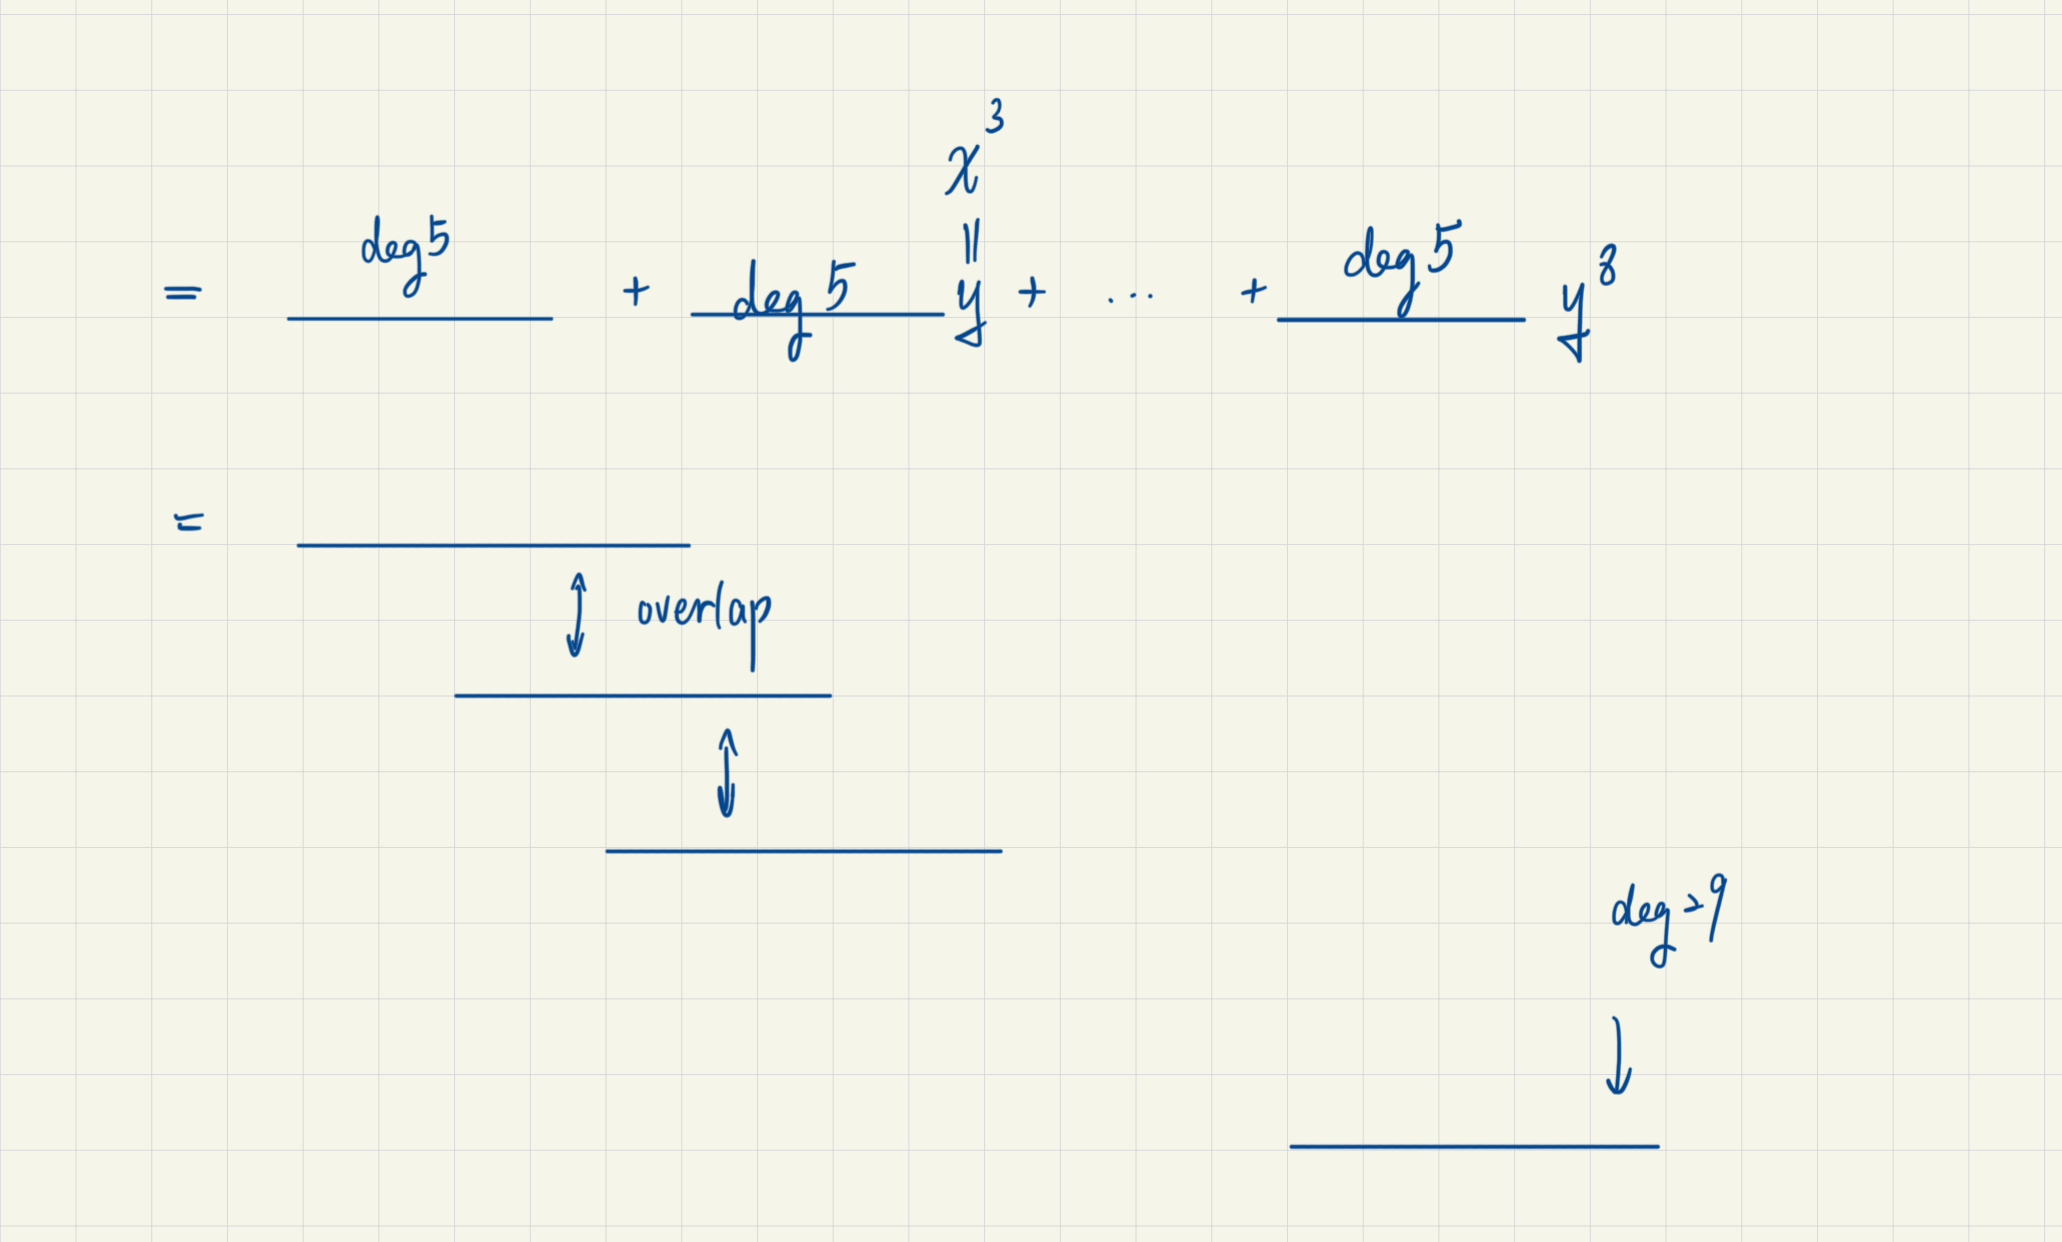
\includegraphics[width = 0.8\textwidth]{Figures/Multilayer1.jpeg}
    \end{center}
\end{frame}



\makepart{Toom-Cook TMVP}

\section{What is TMVP?}
\begin{frame}
    \begin{definition}[Toeplitz Matrix]
        A Toeplitz matrix is the matrix of the form:
        \[
        \begin{bmatrix}
            A_{0} & A_{-1} & \cdots & A_{-(k-1)}\\
            A_{1} & A_{0} & \cdots & A_{-(k-2)}\\
            \vdots & \vdots &\ddots &\vdots \\
            A_{k-1} & A_{k-2} & \cdots & A_{0}\\
        \end{bmatrix}
        \]
    \end{definition}

    \begin{definition}[TMVP Toeplitz Matrix-Vector Product]
        TMVP is a product of a Toeplitz matrix and a column vector
        \[
        \begin{bmatrix}
            A_{0} & A_{-1} & \cdots & A_{-(k-1)}\\
            A_{1} & A_{0} & \cdots & A_{-(k-2)}\\
            \vdots & \vdots &\ddots &\vdots \\
            A_{k-1} & A_{k-2} & \cdots & A_{0}\\
        \end{bmatrix}
        \begin{bmatrix}
            B_{0} \\ B_{1} \\ \vdots \\ B_{k-1}
        \end{bmatrix}.
        \]
    \end{definition}
\end{frame}

\begin{frame}
    Why consider TMVP?

    Recall the definition of weighted convolution, i.e., multiplications in the quotient ring
    \[
        R/\langle x^n - \xi \rangle.
    \]
    If $A = A_{0} + A_{1}x+\cdots+A_{n-1}x^{n-1}$ and $B = B_{0} + B_{1} x + \cdots + B_{n-1} x^{n-1}$, then their product is 
    \[
        C = \sum_{i=0}^{n} C_{i} x^{i}\text{, where }C_{i} = \sum_{k=0}^{i} A_{k}B_{i-k} + \xi\sum_{k=i+1}^{n} A_{k}B_{n+i-k}.
    \]
\end{frame}

\begin{frame}
    Observe that the coefficients of their product
    \[
        C = \sum_{i=0}^{n} C_{i} x^{i}\text{, where }C_{i} = \sum_{k=0}^{i} A_{k}B_{i-k} + \xi\sum_{k=i+1}^{n} A_{k}B_{n+i-k}.
    \]
    can be captured perfectly by a TMVP
    \[
    \begin{bmatrix}
        C_{0} \\ C_{1} \\ \vdots \\ C_{n-1}
    \end{bmatrix}
    \begin{bmatrix}
        A_{0} & \xi A_{n-1} &\cdots & \xi A_{1} \\
        A_{1} & A_{0} &\cdots & \xi A_{2}\\
        \vdots &\vdots & \ddots & \vdots \\
        A_{n-1} & A_{n-2} & \cdots & A_{0}
    \end{bmatrix}
    \begin{bmatrix}
        B_{0} \\ B_{1} \\ \vdots \\ B_{n-1}
    \end{bmatrix}
    \]
    We conclude that if we can compute TMVP efficiently, then we can compute weighted convolution (of course, including cyclic and negacyclic convolution) efficiently.
\end{frame}

\section{Examples of Fast Algorithm}
\begin{frame}
    Now we look at some Fast Algorithm on TMVP:

    Consider decomposing the TMVP $A\cdot B$ as block matrices. Then a two-way decomposition

    \[
\begin{bmatrix}
    \mathbf A_{0} & \mathbf A_{-1}\\
    \mathbf A_{1} & \mathbf A_{0}
\end{bmatrix}
\begin{bmatrix}
    \mathbf B_{0} \\ \mathbf B_{1}
\end{bmatrix}
=
\begin{bmatrix}
    \mathbf A_{0} \mathbf B_{0} + \mathbf A_{-1} \mathbf B_{1} \\
    \mathbf A_{1} \mathbf B_{0} + \mathbf A_{0} \mathbf B_{1} 
\end{bmatrix}
=
\begin{bmatrix}
    (\mathbf A_{0} + \mathbf A_{-1}) \mathbf B_{1} + \mathbf A_{0} (\mathbf B_{0} - \mathbf B_{1})
    \\ 
    (\mathbf A_{1} + \mathbf A_{0}) \mathbf B_{0} - \mathbf A_{0} (\mathbf B_{0} - \mathbf B_{1})
\end{bmatrix}
    \]

    and a three way decomposition:

    \[
\begin{aligned}
    \begin{bmatrix}
        \mathbf A_{0} & \mathbf A_{-1} & \mathbf A_{-2} \\
        \mathbf A_{1} & \mathbf A_{0} & \mathbf A_{-1} \\
        \mathbf A_{2} & \mathbf A_{1} & \mathbf A_{0} \\
    \end{bmatrix}
    \begin{bmatrix}
        \mathbf B_{0} \\ \mathbf B_{1} \\ \mathbf B_{2}
    \end{bmatrix}
    &=
    \begin{bmatrix}
        \mathbf{A}_{0} \mathbf{B}_{0} + \mathbf{A}_{-1} \mathbf{B}_{1} + \mathbf{A}_{-2} \mathbf{B}_{2} \\
        \mathbf{A}_{1} \mathbf{B}_{0} + \mathbf{A}_{0} \mathbf{B}_{1} + \mathbf{A}_{-1} \mathbf{B}_{2} \\
        \mathbf{A}_{2} \mathbf{B}_{0} + \mathbf{A}_{1} \mathbf{B}_{1} + \mathbf{A}_{0} \mathbf{B}_{2}
    \end{bmatrix}
    \\
    &=
    \begin{bmatrix}
        \left(\mathbf{A}_{0} + \mathbf{A}_{-1} + \mathbf{A}_{-2}\right)\mathbf B_{2} 
        + \mathbf A_{-1} (\mathbf B_{1} - \mathbf B_{2}) - \mathbf A_{0} (\mathbf B_{2} - \mathbf B_{0})
        \\
        \left(\mathbf{A}_{1} + \mathbf{A}_{0} + \mathbf{A}_{-1}\right)\mathbf B_{1}   
        + \mathbf A_{1} (\mathbf B_{0}- \mathbf B_{1}) - \mathbf A_{-1} (\mathbf B_{1} - \mathbf B_{2})
        \\
        \left(\mathbf{A}_{2} + \mathbf{A}_{1} + \mathbf{A}_{0} \right)\mathbf B_{0}
        + \mathbf A_{0} (\mathbf B_{2}-\mathbf B_{0}) - \mathbf A_{1} (\mathbf B_{0} - \mathbf B_{1})
    \end{bmatrix}
\end{aligned}
\]

The three way decomposition formula allow us to complete the full TMVP with only six $\frac13$-size TMVP.
\end{frame}

\begin{frame}
    However, there exists a fast algorithm that completes the full TMVP with only five $\frac13$-size TMVP:
    \[
    \begin{aligned}
    & P_0=\left(-A_0+\frac{1}{2} A_{-1}-\frac{1}{2} A_1+A_2\right)B_{0} \\
    & P_1=\left(\frac{1}{2} A_0-\frac{1}{2} A_{-1}+A_1\right)\left(B_{0} + B_{1} + B_{2}\right) \\
    & P_2=\left(\frac{1}{2} A_0-\frac{1}{6} A_{-1}-\frac{1}{3} A_1\right)\left(B_{0}-B_{1}+B_{2}\right) \\
    & P_3=\left(\frac{1}{6} A_{-1}-\frac{1}{6} A_1\right)\left(B_{0} + 2B_{1}+4B_{2}\right) \\
    & P_4=\left(-A_0-2 A_{-1}+A_{-2}+2 A_1\right)\left(B_{2}\right)
    \end{aligned}
    \]
    and
    \[
    \begin{bmatrix}
        A_{0} & A_{-1} & A_{-2}\\
        A_{1} & A_{0} & A_{-1}\\
        A_{2} & A_{1} & A_{0}
    \end{bmatrix}
    \begin{bmatrix}
        B_{0} \\ B_{1} \\ B_{2}
    \end{bmatrix}
    =
    \begin{bmatrix}
        P_{0} + P_{1} + P_{2} + P_{3}\\
        P_{1} - P_{2} + 2 P_{3}\\
        P_{1} + P_{2} + 4P_{3}+P_{4}
    \end{bmatrix}
    \]
    In the next section, we derive a general procedure that completes the full TMVP by $2k-1$ $\frac{1}{k}$-size TMVP.
\end{frame}




\section{Derivation of Toom-Cook-3 Fast Algorithm}

\begin{frame}
    We first derive the above mentioned 3-way TMVP.
    The coefficients suggest that the derivation of that formula is heavily related to Toom-Cook multiplication.

    Let's recall the Toom-Cook-3 multiplication:
    \[
    R= 
    \mathbf{TC}_{5\times 5}^{-1} \left(
        \left(\mathbf{TC}_{5\times 3} B\right)
        \odot
        \left(\mathbf{TC}_{5\times 3} C\right)
    \right)
    \]
    First we note that 
    \[
    R = 
    \begin{bmatrix}
        R_{0} \\ R_{1} \\ R_{2} \\ R_{3} \\ R_{4}
    \end{bmatrix}
    =\begin{bmatrix}
        B_{0}C_{0} \\ 
        B_{1}C_{0} &+&B_{0}C_{1} \\
        B_{2}C_{0} &+&B_{1}C_{1} &+& B_{0}C_{2} \\
                   &&B_{2}C_{1} &+& B_{1}C_{2} \\
                               &&&& B_{2}C_{2}
    \end{bmatrix}
    \]
\end{frame}

\begin{frame}
    Multiply this $R$ vector by $\vec{A} = \begin{bmatrix}A_{2} & A_{1} & A_{0} & A_{-1} & A_{-2}\end{bmatrix}$.
    \[
        \begin{bmatrix}A_{2} & A_{1} & A_{0} & A_{-1} & A_{-2}\end{bmatrix}
        \begin{bmatrix}
            B_{0}C_{0} \\ 
            B_{1}C_{0} &+&B_{0}C_{1} \\
            B_{2}C_{0} &+&B_{1}C_{1} &+& B_{0}C_{2} \\
                       &&B_{2}C_{1} &+& B_{1}C_{2} \\
                                   &&&& B_{2}C_{2}
        \end{bmatrix}
    \]
    Then we have:
    \[
    \begin{aligned}
        \text{coefficient of } C_{0} &= A_{2}B_{0} + A_{1}B_{1} + A_{0}B_{2}\\
        \text{coefficient of } C_{1} &= A_{1}B_{0} + A_{0}B_{1} + A_{-1}B_{2}\\
        \text{coefficient of } C_{2} &= A_{0}B_{0} + A_{-1}B_{1} + A_{-2}B_{2}
    \end{aligned}
    \]
    which is just the reversed column vector of
    \[
    \begin{bmatrix}
        A_{0} & A_{-1} & A_{-2}\\
        A_{1} & A_{0} & A_{-1}\\
        A_{2} & A_{1} & A_{0}
    \end{bmatrix}
    \begin{bmatrix}
        B_{0} \\ B_{1} \\ B_{2}
    \end{bmatrix}
    =
    \begin{bmatrix}
        A_{0}B_{0} + A_{-1}B_{1} + A_{-2}B_{2}\\
        A_{1}B_{0} + A_{0}B_{1} + A_{-1}B_{2}\\
        A_{2}B_{0} + A_{1}B_{1} + A_{0}B_{2}
    \end{bmatrix}
    \]
\end{frame}

\begin{frame}
    Hence in right hand side,
    \[
    \vec{A} \mathbf{TC}_{5\times 5}^{-1} \left(\left(\mathbf{TC}_{5\times 3}B\right)\odot \left(\mathbf{TC}_{5\times 3}C\right)\right)
    \]
    its $C_0$ entry, $C_1$ entry and $C_2$ entry are reversed column vector elements of 
    \[
    \begin{bmatrix}
        A_{0} & A_{-1} & A_{-2}\\
        A_{1} & A_{0} & A_{-1}\\
        A_{2} & A_{1} & A_{0}
    \end{bmatrix}
    \begin{bmatrix}
        B_{0} \\ B_{1} \\ B_{2}
    \end{bmatrix}
    =
    \begin{bmatrix}
        A_{0}B_{0} + A_{-1}B_{1} + A_{-2}B_{2}\\
        A_{1}B_{0} + A_{0}B_{1} + A_{-1}B_{2}\\
        A_{2}B_{0} + A_{1}B_{1} + A_{0}B_{2}
    \end{bmatrix}
    \]
    Let's focus on $C_0$'s coefficients, it is finded by letting $C_0=1$ and $C_\text{others}=0$:
    \[
    C_{0}\text{'s coefficient} = \vec{A} \mathbf{TC}_{5\times 5}^{-1} \left(\left(\mathbf{TC}_{5\times 3}\begin{bmatrix}B_{0}\\B_{1}\\B_{2}\end{bmatrix}\right)\odot \left(\mathbf{TC}_{5\times 3}\begin{bmatrix}1\\0\\0\end{bmatrix}\right)\right)
    \]
\end{frame}


\begin{frame}
    \[
    C_{0}\text{'s coefficient} = \vec{A} \mathbf{TC}_{5\times 5}^{-1} \left(\left(\mathbf{TC}_{5\times 3}\begin{bmatrix}B_{0}\\B_{1}\\B_{2}\end{bmatrix}\right)\odot \left(\mathbf{TC}_{5\times 3}\begin{bmatrix}1\\0\\0\end{bmatrix}\right)\right)
    \]
    and similarly
    \[
    C_{1}\text{'s coefficient} = \vec{A} \mathbf{TC}_{5\times 5}^{-1} \left(\left(\mathbf{TC}_{5\times 3}\begin{bmatrix}B_{0}\\B_{1}\\B_{2}\end{bmatrix}\right)\odot \left(\mathbf{TC}_{5\times 3}\begin{bmatrix}0\\1\\0\end{bmatrix}\right)\right)
    \]
    \[
    C_{2}\text{'s coefficient} = \vec{A} \mathbf{TC}_{5\times 5}^{-1} \left(\left(\mathbf{TC}_{5\times 3}\begin{bmatrix}B_{0}\\B_{1}\\B_{2}\end{bmatrix}\right)\odot \left(\mathbf{TC}_{5\times 3}\begin{bmatrix}0\\0\\1\end{bmatrix}\right)\right)
    \]
\end{frame}

\begin{frame}
    \[
    C_{0}\text{'s coefficient} = \vec{A} \mathbf{TC}_{5\times 5}^{-1} \left(\left(\mathbf{TC}_{5\times 3}\begin{bmatrix}B_{0}\\B_{1}\\B_{2}\end{bmatrix}\right)\odot \left( \begin{bmatrix}1\\1\\1\\1\\0\end{bmatrix} \right)\right)
    \]
    \[
    C_{1}\text{'s coefficient} = \vec{A} \mathbf{TC}_{5\times 5}^{-1} \left(\left(\mathbf{TC}_{5\times 3}\begin{bmatrix}B_{0}\\B_{1}\\B_{2}\end{bmatrix}\right)\odot \left( \begin{bmatrix}0\\1\\-1\\2\\0\end{bmatrix} \right)\right)
    \]
    \[
    C_{2}\text{'s coefficient} = \vec{A} \mathbf{TC}_{5\times 5}^{-1} \left(\left(\mathbf{TC}_{5\times 3}\begin{bmatrix}B_{0}\\B_{1}\\B_{2}\end{bmatrix}\right)\odot \left( \begin{bmatrix}0\\1\\1\\4\\1\end{bmatrix} \right)\right)
    \]
\end{frame}


\begin{frame}
    Let $e_{0} = \begin{bmatrix}1\\0\\0\\0\\0\end{bmatrix}$ and $e_{1} = \begin{bmatrix}0\\1\\0\\0\\0\end{bmatrix}$, etc..
    Then
    \[
        C_{0}\text{'s coefficient} = \vec{A} \mathbf{TC}_{5\times 5}^{-1} \left(\left(\mathbf{TC}_{5\times 3}\begin{bmatrix}B_{0}\\B_{1}\\B_{2}\end{bmatrix}\right)\odot \left( \begin{bmatrix}1\\1\\1\\1\\0\end{bmatrix} \right)\right)
    \]
    can be rewritten as
    \[
        C_{0}\text{'s coefficient} = \vec{A} \mathbf{TC}_{5\times 5}^{-1} 
        \left(\left(\mathbf{TC}_{5\times 3}\begin{bmatrix}B_{0}\\B_{1}\\B_{2}\end{bmatrix}\right)\odot (e_{0}+e_{1}+e_{2}+e_{3}) \right)
    \]
\end{frame}
\begin{frame}
    And by linearity
    \[\begin{aligned}
            C_{0}\text{'s coefficient} &= \vec{A} \mathbf{TC}_{5\times 5}^{-1} 
            \left(\left(\mathbf{TC}_{5\times 3}\begin{bmatrix}B_{0}\\B_{1}\\B_{2}\end{bmatrix}\right)\odot e_{0} \right)
            +
            \vec{A} \mathbf{TC}_{5\times 5}^{-1} 
            \left(\left(\mathbf{TC}_{5\times 3}\begin{bmatrix}B_{0}\\B_{1}\\B_{2}\end{bmatrix}\right)\odot e_{1} \right)
            \\&+
            \vec{A} \mathbf{TC}_{5\times 5}^{-1} 
            \left(\left(\mathbf{TC}_{5\times 3}\begin{bmatrix}B_{0}\\B_{1}\\B_{2}\end{bmatrix}\right)\odot e_{2} \right)
            +
            \vec{A} \mathbf{TC}_{5\times 5}^{-1} 
            \left(\left(\mathbf{TC}_{5\times 3}\begin{bmatrix}B_{0}\\B_{1}\\B_{2}\end{bmatrix}\right)\odot e_{3} \right)
    \end{aligned}
    \]
    Hence we conclude that each of three coefficients can be written as a linear combination of the following materials
    \[
        \vec{A} \mathbf{TC}_{5\times 5}^{-1} 
        \left(\left(\mathbf{TC}_{5\times 3}\begin{bmatrix}B_{0}\\B_{1}\\B_{2}\end{bmatrix}\right)\odot e_{i} \right)
        \text{ for }i=0,1,2,3,4.
    \]
    And it follows that five $\frac13$-size TMVP are sufficient for the full TMVP.
\end{frame}


\begin{frame}
    We go through the detailed computation of TMVP-TC-3.
Put
\[
\mathrm{COMPONENT} = 
\begin{bmatrix}
        \vec{A} \mathbf{TC}_{5\times 5}^{-1} 
        \left(\left(\mathbf{TC}_{5\times 3}\begin{bmatrix}B_{0}\\B_{1}\\B_{2}\end{bmatrix}\right)\odot e_{0} \right)\\
        \vec{A} \mathbf{TC}_{5\times 5}^{-1} 
        \left(\left(\mathbf{TC}_{5\times 3}\begin{bmatrix}B_{0}\\B_{1}\\B_{2}\end{bmatrix}\right)\odot e_{1} \right)\\
        \vec{A} \mathbf{TC}_{5\times 5}^{-1} 
        \left(\left(\mathbf{TC}_{5\times 3}\begin{bmatrix}B_{0}\\B_{1}\\B_{2}\end{bmatrix}\right)\odot e_{2} \right)\\
        \vec{A} \mathbf{TC}_{5\times 5}^{-1} 
        \left(\left(\mathbf{TC}_{5\times 3}\begin{bmatrix}B_{0}\\B_{1}\\B_{2}\end{bmatrix}\right)\odot e_{3} \right)\\
        \vec{A} \mathbf{TC}_{5\times 5}^{-1} 
        \left(\left(\mathbf{TC}_{5\times 3}\begin{bmatrix}B_{0}\\B_{1}\\B_{2}\end{bmatrix}\right)\odot e_{4} \right)
\end{bmatrix}
\]


\end{frame}
\begin{frame}
    Then

    \[
        \begin{bmatrix}
            A_{0}B_{0} + A_{-1}B_{1} + A_{-2}B_{2}\\
            A_{1}B_{0} + A_{0}B_{1} + A_{-1}B_{2}\\
            A_{2}B_{0} + A_{1}B_{1} + A_{0}B_{2}
        \end{bmatrix}
        =
        \underbrace{\begin{bmatrix}
            &&1\\
            &1&\\
            1&&
        \end{bmatrix}}_{\text{reverse}}
        \underbrace{\begin{bmatrix}
            1 & 1 & 1 & 1 & 0\\
            0 & 1 & -1 & 2 &0\\
            0 & 1 & 1 & 4 & 1
        \end{bmatrix}}_{\mathbf{TC}_{5\times 3}^T}
        \mathrm{COMPONENT}.
    \]
\end{frame}

\section{Derivation of Toom-Cook-$k$ Fast Algorithm}
\begin{frame}
    We now want to generalize our idea to $k$-way decomposition formula for
    \[
    \begin{bmatrix}
        A_{0} & A_{-1} & \cdots &A_{-(k-1)}\\
        A_{1} & A_{0} & \cdots &A_{-(k-2)}\\
        \vdots & \vdots & \ddots & \vdots\\
        A_{k-1} & A_{k-1} & \cdots &A_{0}\\
    \end{bmatrix}
    \begin{bmatrix}
        B_{0} \\ B_{1} \\ \vdots \\ B_{k-1}
    \end{bmatrix}.
    \]

\end{frame}
\begin{frame}
    Begin from the Toom-Cook multiplication:
    \[
    R=\mathbf{TC}_{(2k-1)\times (2k-1)}^{-1}\left(
        \left(\mathbf{TC}_{(2k-1)\times k}B\right)\odot
        \left(\mathbf{TC}_{(2k-1)\times k}C\right)
    \right)
    \]
    Multiply the both sides by the row vector
    \[
    \vec{A} = \begin{bmatrix} A_{k-1} & A_{k-2} & \cdots & A_{-(k-1)}\end{bmatrix}.
    \]
\end{frame}

\begin{frame}
    Let's look at the $C_{i_0}$ coefficient of the left-hand side
    \[
    C_{i_0}\text{'s coefficient}
    =
    A_{-k+i_{0}+1}B_{0} + A_{-k+i_{0}+2}B_{1} + \cdots + A_{i_{0}} B_{k-1}
    \]
    which is the last $i$th component of in the
    \[
    \begin{bmatrix}
        A_{0} & A_{-1} & \cdots &A_{-(k-1)}\\
        A_{1} & A_{0} & \cdots &A_{-(k-2)}\\
        \vdots & \vdots & \ddots & \vdots\\
        A_{k-1} & A_{k-1} & \cdots &A_{0}\\
    \end{bmatrix}
    \begin{bmatrix}
        B_{0} \\ B_{1} \\ \vdots \\ B_{k-1}
    \end{bmatrix}.
    \]

\end{frame}



\begin{frame}
    So the $C_{i_0}$'s coefficient of the
    \[
        \vec{A}\mathbf{TC}_{(2k-1)\times (2k-1)}^{-1}\left(
            \left(\mathbf{TC}_{(2k-1)\times k}B\right)\odot
            \left(\mathbf{TC}_{(2k-1)\times k}C\right)
        \right)
    \]
    is the last $i$th component of in the
    \[
        \begin{bmatrix}
        A_{0} & A_{-1} & \cdots &A_{-(k-1)}\\
        A_{1} & A_{0} & \cdots &A_{-(k-2)}\\
        \vdots & \vdots & \ddots & \vdots\\
        A_{k-1} & A_{k-1} & \cdots &A_{0}\\
        \end{bmatrix}
        \begin{bmatrix}
        B_{0} \\ B_{1} \\ \vdots \\ B_{k-1}
        \end{bmatrix}.
    \]

\end{frame}

\begin{frame}
    The $C_{i_0}$'s coefficient of the
    \[
        \vec{A}\mathbf{TC}_{(2k-1)\times (2k-1)}^{-1}\left(
            \left(\mathbf{TC}_{(2k-1)\times k}B\right)\odot
            \left(\mathbf{TC}_{(2k-1)\times k}C\right)
        \right)
    \]    
    is
    \[
        \vec{A}\mathbf{TC}_{(2k-1)\times (2k-1)}^{-1}\left(
            \left(\mathbf{TC}_{(2k-1)\times k}B\right)\odot
            {\left(\mathbf{TC}_{(2k-1)\times k}\begin{bmatrix}
                0\\\vdots \\ 1 \\ \vdots \\0
            \end{bmatrix}\right)}
        \right).
    \]
\end{frame}


\begin{frame}
    \[
        \vec{A}\mathbf{TC}_{(2k-1)\times (2k-1)}^{-1}\left(
            \left(\mathbf{TC}_{(2k-1)\times k}B\right)\odot
            \textcolor{blue}{\left(\mathbf{TC}_{(2k-1)\times k}\begin{bmatrix}
                0\\\vdots \\ 1 \\ \vdots \\0
            \end{bmatrix}\right)}
        \right).
    \]
    By multiplying the blue part out, we can again write this expression as a linear combination of
    \[
        \vec{A}\mathbf{TC}_{(2k-1)\times (2k-1)}^{-1}\left(
            \left(\mathbf{TC}_{(2k-1)\times k}B\right)\odot
            e_{i}
        \right)\text{ for }i=0,1,\ldots,2k-2
    \]
    From here, we conclude that we can perform the full TMVP computation by computing $2k-1$ $\frac{1}{k}$-size TMVP.

\end{frame}


\section{Final Remark}
\begin{frame}

        The speed up of ratio
        \[\frac{k^{2}}{2k-1}\]
        looks very good. 
        But please note that the formula is based on Toom-Cook multiplication which involves choosing $\{s_{i}\}$, the interpolation points.
        When we choose a large $k$, the resulting $\mathbf{TC}$ and $\mathbf{TC}^{-1}$ matrices will be complicated and hence slow down the process.

        In the paper, two multiplication methods in the ring
        \[
        \mathbb{Z}_{2048}/\left\langle x^{677}-1\right\rangle
        \]
        are proposed:
        
        Multilayer Toom-Cook and Multilayer TMVP-Toom-Cook both with the splitting sequence 5 -> 3 -> 3 -> 2.

\end{frame}



\begin{frame}
    
\end{frame}

\end{document}